\subsection{Estrutura de um Clock de Redstone}

No contexto do Minecraft, o clock é implementado por meio de circuitos de redstone que exploram atrasos discretos introduzidos por componentes como repetidores.

Diferentemente de circuitos eletrônicos físicos, nos quais o tempo é contínuo e os atrasos são fenômenos analógicos, o tempo no jogo é explicitamente quantizado em \textit{ticks}, conforme definido anteriormente. Dessa forma, tanto a propagação de sinais quanto a atualização de estados ocorrem em múltiplos inteiros de Game Ticks (GT) ou Redstone Ticks (RT).

Neste projeto, será utilizado um loop de repetidores de redstone que introduzem um atraso $\tau$ cada, em Redstone Ticks, de forma qual um pulso percorre continuamente um caminho fechado. 

Como no jogo não existe dispersão de energia do sistema ressonante, o sinal permanece indefinidamente, produzindo uma oscilação periódica cujo período $T$ é determinado pela soma dos atrasos introduzidos ao longo do circuito. Dessa forma, para melhor controle do período, serão utilizados os repetidores do mod \textit{Wired Redstone}.

\begin{figure}[H]
    \centering
    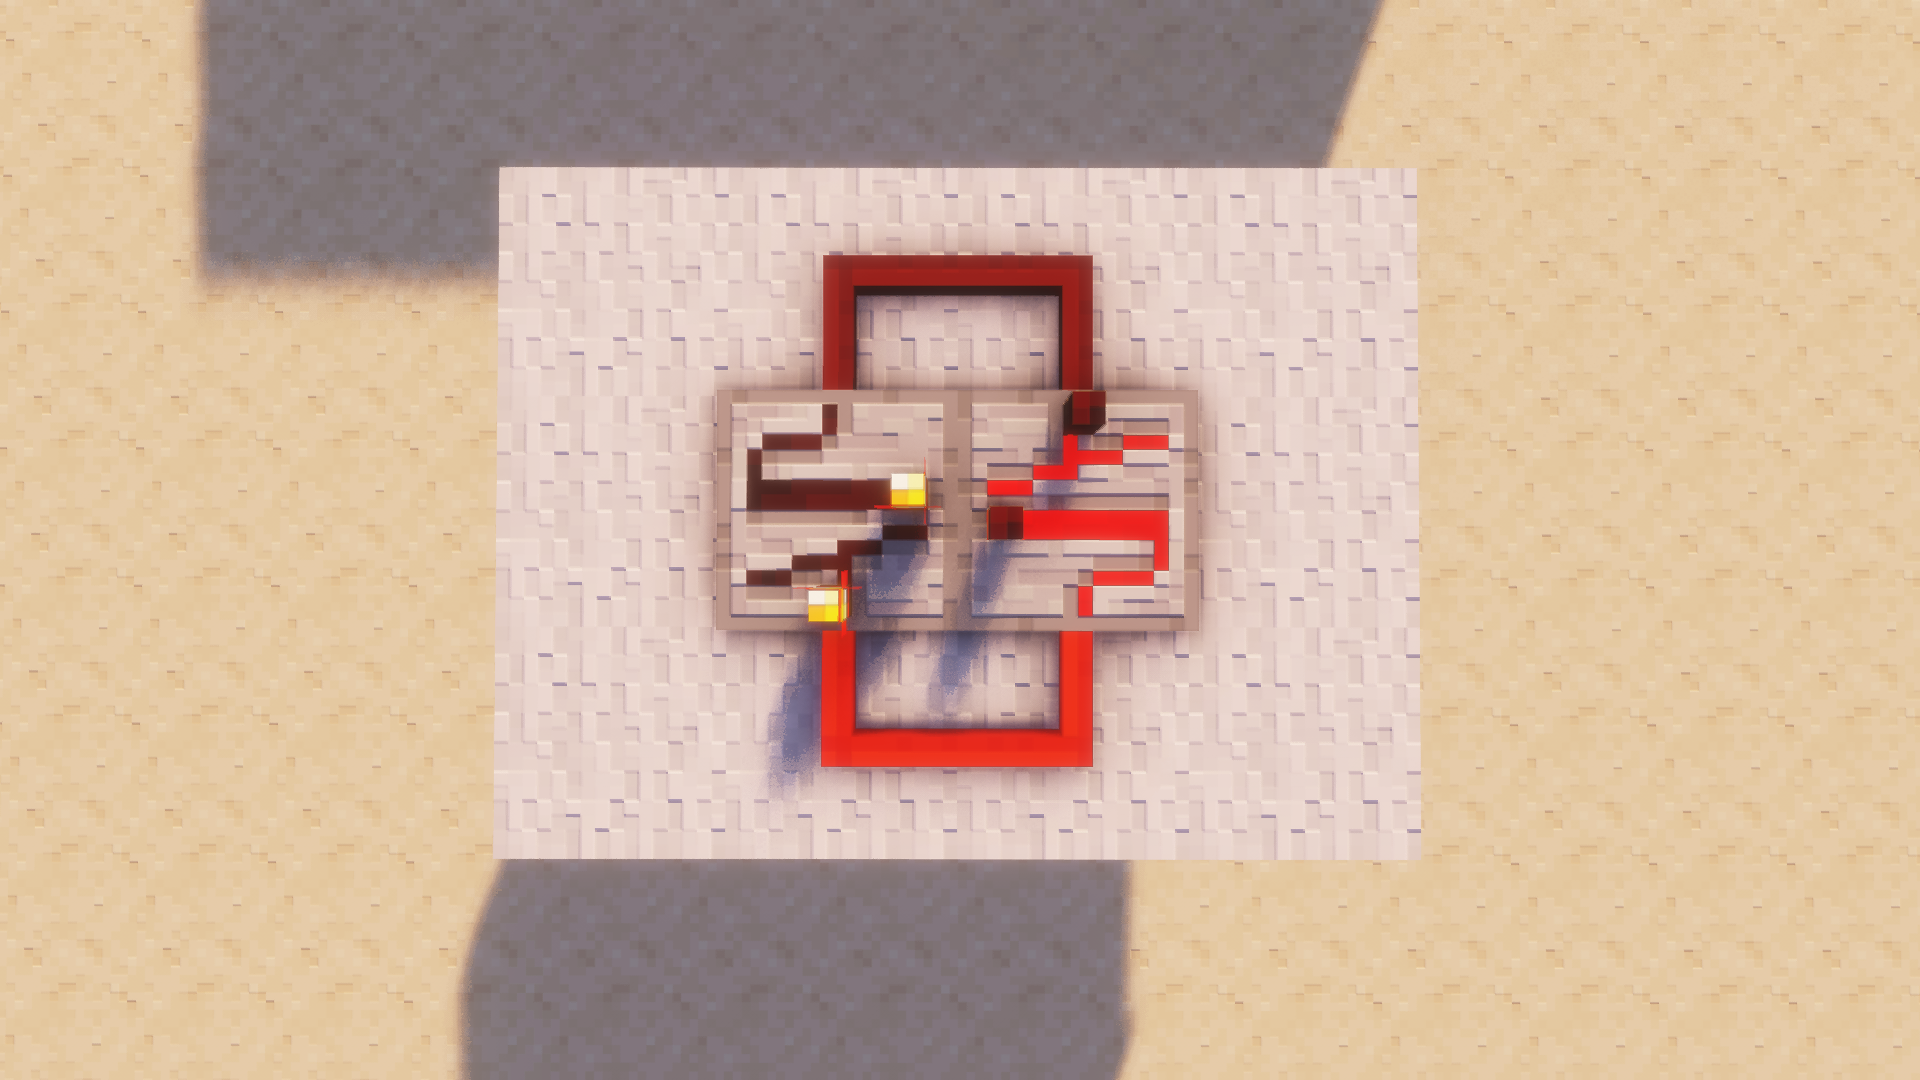
\includegraphics[width=0.7\linewidth]{images/clock-redstone.png}
    \caption{Clock no Minecraft}
    \label{fig:clock-redstone}
\end{figure}

Esta implementação, entretanto, possúi um problema central: não é possível desativar e reativar as oscilações. Portanto, um dos repetidores será substituido por uma porta AND, a qual introduz atraso $\alpha$ RTs, que receberá um bit $A$, de tal forma que para $A = 0$ o ciclo será aberto, atuando como um controlador/transistor/amplificador do sistema.  

\begin{figure}[H]
    \centering
    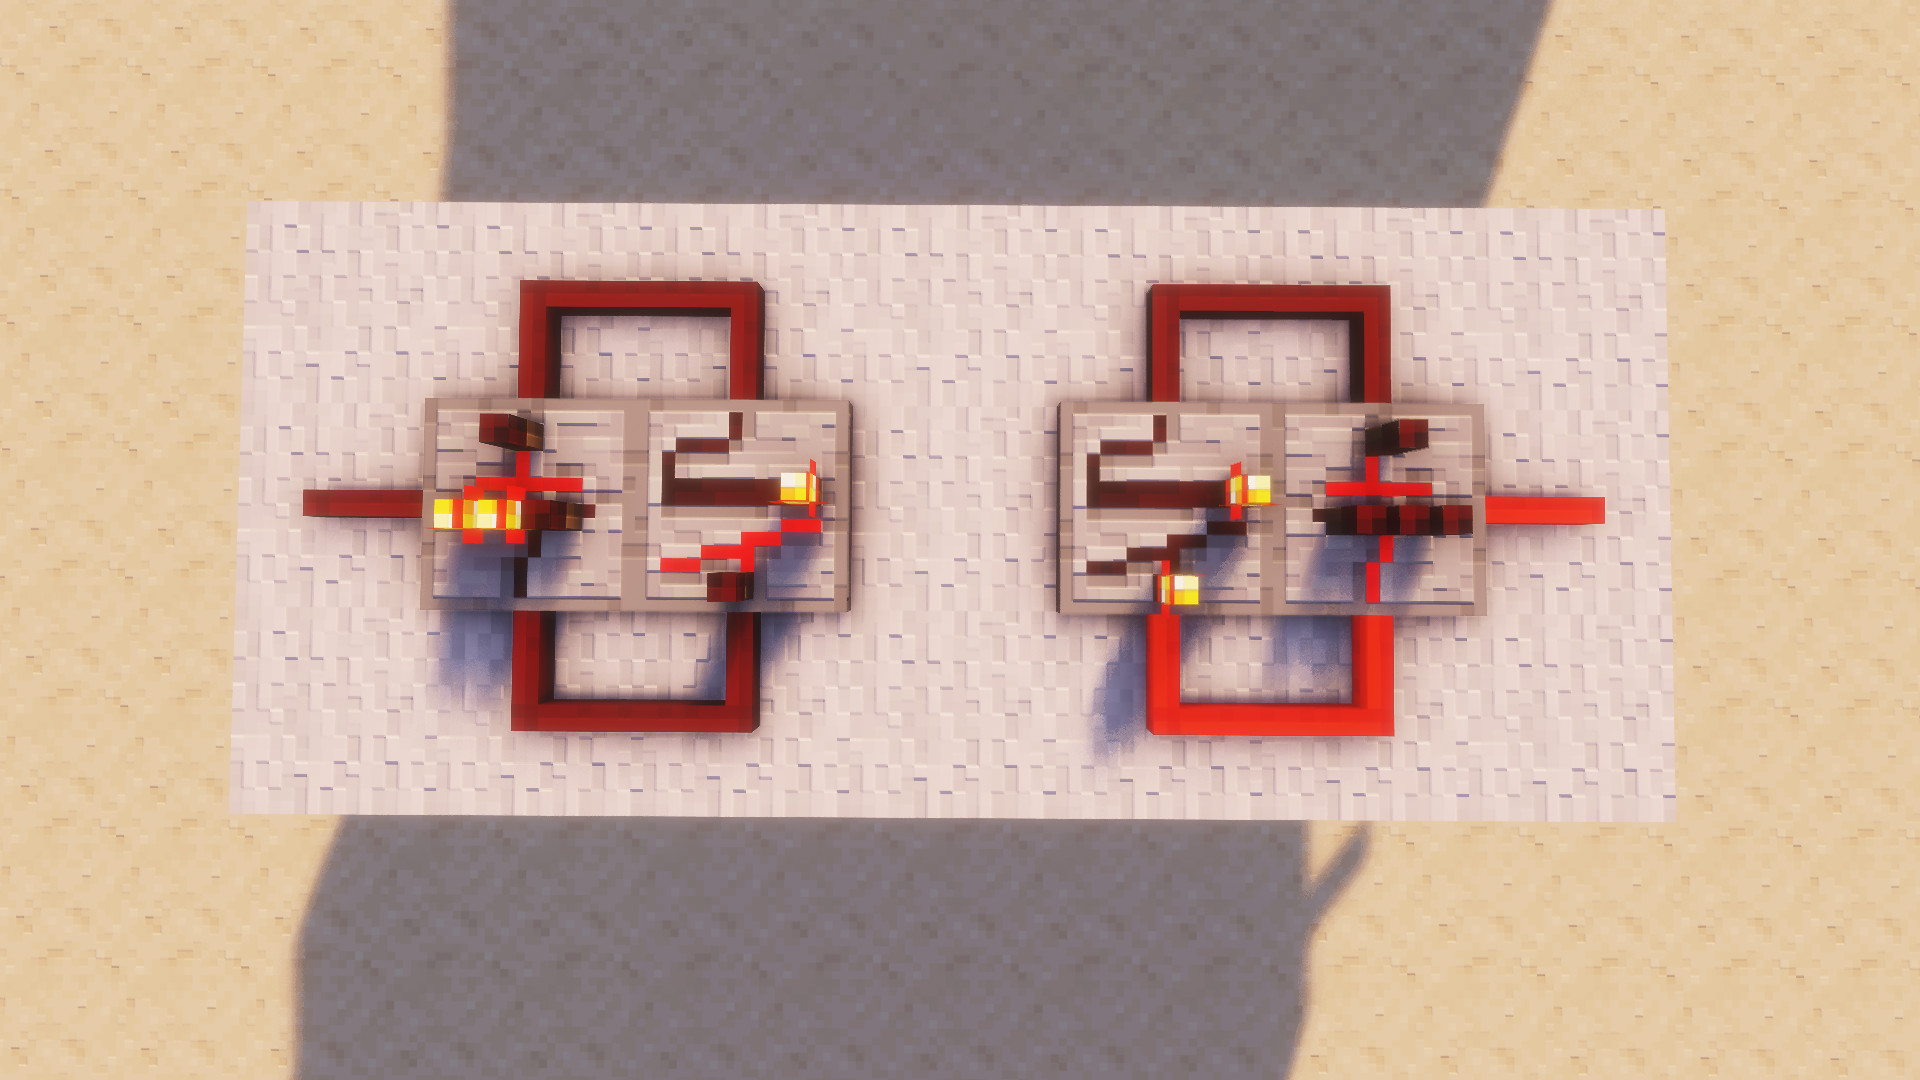
\includegraphics[width=0.7\linewidth]{images/clock-redstone-controlado.png}
    \caption{Clock no Minecraft com controle A}
    \label{fig:clock-redstone-controlado}
\end{figure}

A retomada das oscilações requer a injeção de um pulso inicial no circuito. Esse pulso atua como uma perturbação que passa a circular no loop, estabelecendo o regime periódico.

Para que o sistema opere corretamente, é necessário que exista apenas um único pulso propagando-se ao longo do circuito. Caso o pulso de ativação seja excessivamente longo, ele pode ocupar múltiplos estágios simultaneamente, resultando na formação de múltiplos pulsos no loop e, consequentemente, em comportamento incorreto do clock.

Seja $w$ a largura do pulso de ativação. Para garantir a propagação de um único pulso, deve-se impor a seguinte condição:

\[
w < \min(\tau, \alpha)
\]

onde $\tau$ representa o atraso dos repetidores e $\alpha$ o atraso introduzido pela porta de controle.

Essa restrição assegura que o pulso não se estenda por mais de um elemento do circuito ao mesmo tempo, preservando a integridade da oscilação periódica.